\begin{figure}[t!]
\centering
%\vspace{-10px}
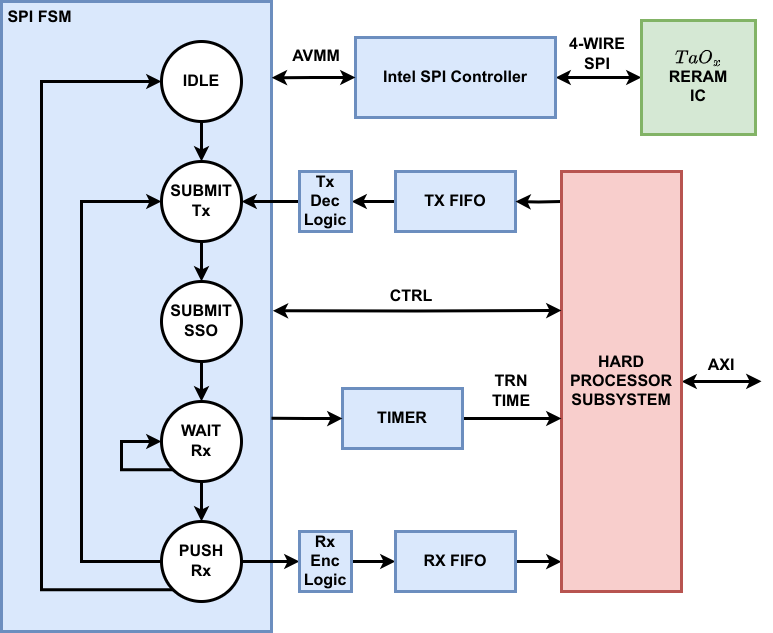
\includegraphics[width=0.6\linewidth]{img/spi_time_sys.png}
\caption{A ReRAM timing characterization system. An Intel FPGA SPI controller core drives a 4-wire SPI master interface to a Click2ReRAM module containing a Fujitsu MB85AS8MT TaOX 8Mb ReRAM memory. An ARM A9 hard processor system drives a test pattern to the TX FIFO. A SPI FSM core pops test patterns off of the FIFO and drives them to the SPI controller at the ReRAM F$_{max}$ of 10MHz and concurrently starts a fine-grained timer running at the system clock of 100MHz. The SPI FSM polls the ReRAM module for a completion flag through the SPI core. The controller module supports read and write transactions. Reads do not provide timing data, as all reads complete in one SPI transaction.}
\label{fig:reram_measurement_sys}
\end{figure} 
